\documentclass[a4paper]{article}
\usepackage[warn]{mathtext}
\usepackage[utf8]{inputenc}
\usepackage[T2A]{fontenc}
\usepackage[english,russian]{babel}
\usepackage{indentfirst}
\usepackage{misccorr}
\usepackage{subcaption}
\captionsetup{compatibility=false}
\usepackage{geometry}
\geometry{verbose,a4paper,tmargin=2cm,bmargin=2cm,lmargin=1.5cm,rmargin=1.5cm}
\usepackage{graphicx}
\usepackage{wrapfig}
\usepackage{amsmath}
\usepackage{fancyhdr}
\usepackage{floatflt}
\usepackage{float}
\usepackage{amssymb}
\usepackage{color}
\usepackage{lscape}
\usepackage{hvfloat}
\usepackage{amsfonts}
\usepackage{euscript}
\usepackage{newunicodechar}

\begin{document}

\begin{titlepage}
	\centering
	\vspace{5cm}
	{\scshape\LARGE Московский физико-технический институт \par}

	\vspace{3cm}
	{\scshape\Large Лабораторная работа № 4.3.1 \par}
	\vspace{1cm}
	{\huge\bfseries  Изучение дифракции света\par}
	\vspace{1cm}
	\vfill
\begin{flushright}
	{\large Выполнила студентка группы Б01-903}\par
	\vspace{0.3cm}
	{\LARGE Прохорова Юлия}
\end{flushright}
	
	\vfill

% Bottom of the page
	Долгопрудный, 2021 г.
\end{titlepage}



\newpage

%\tableofcontents

\newpage

\newcommand{\RNumb}[1]{\uppercase\expandafter{\romannumeral #1\relax}}

\pagestyle{fancy} 
\fancyhead{} 
\fancyhead[R]{Юлия Прохорова, Б01-903} 
\fancyhead[L]{4.3.1}
\fancyfoot[C]{\noindent\rule{\textwidth}{0.4pt} \thepage}

\paragraph*{Цель работы:} исследовать явления дифракции Френеля и Фраунгофера на щели, изучить влияние дифракции на разрешающую способность оптических инструментов.
	
\paragraph*{Оборудование:} оптическая скамья, ртутная лампа, монохроматор, щели с регулируемой шириной, рамка с вертикальной
нитью, двойная щель, микроскоп на поперечных салазках с микрометрическим винтом, зрительная труба.

\section{Теоретическая часть}
	
\subsection{Дифракция Френеля на щели}
	
Световые лучи освещают щель $S_2$ и испытывают на ней дифракцию. Дифракционная картина рассматривается с помощью микроскопа М, сфокусированного на некоторую
плоскость наблюдения П.

	\begin{figure}[h!]
		\centering
		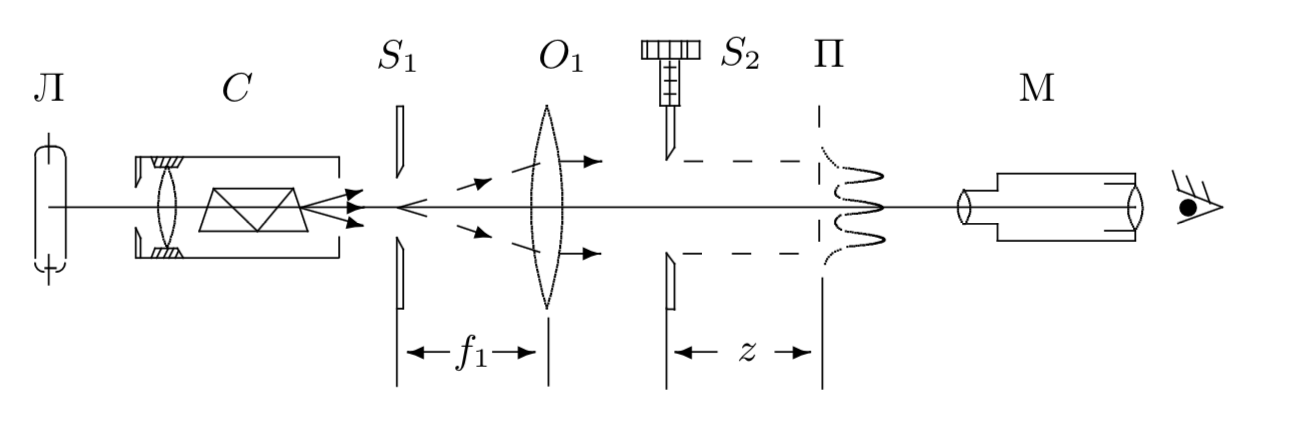
\includegraphics[width=0.8\linewidth]{a.png}
		\caption{Схема установки для наблюдения дифракции Френеля}
		\label{labA}
	\end{figure}

	Суммарная ширина $m$ зон Френеля $z_m$ определяется соотношением:
	
	\begin{equation}
		z_m = \sqrt{am\lambda} \label{sum}
	\end{equation}

	где $a$ — расстояние от щели до плоскости наблюдения (рис. 1), а $\lambda = 546 $ нм — длина волны. Вид
	наблюдаемой дифракционной картины определяется числом Френеля $\varPhi$: квадрат числа
	Френеля - это отношение ширины щели $D$ к размеру первой зоны Френеля, т.е. число зон
	Френеля, которые укладываются на ширине щели.

\begin{equation}\label{xin}
Ф^2 = \frac{D}{\sqrt{a\lambda}}
\end{equation}

Обратную величину называют \textbf{волновым параметром}:

\begin{equation}\label{xin}
	P = \frac{1}{Ф^2} = \frac{\sqrt{a\lambda}}{D}
\end{equation}

\subsection{Дифракция Фраунгофера на щели}


\begin{figure}[H]
	\centering
	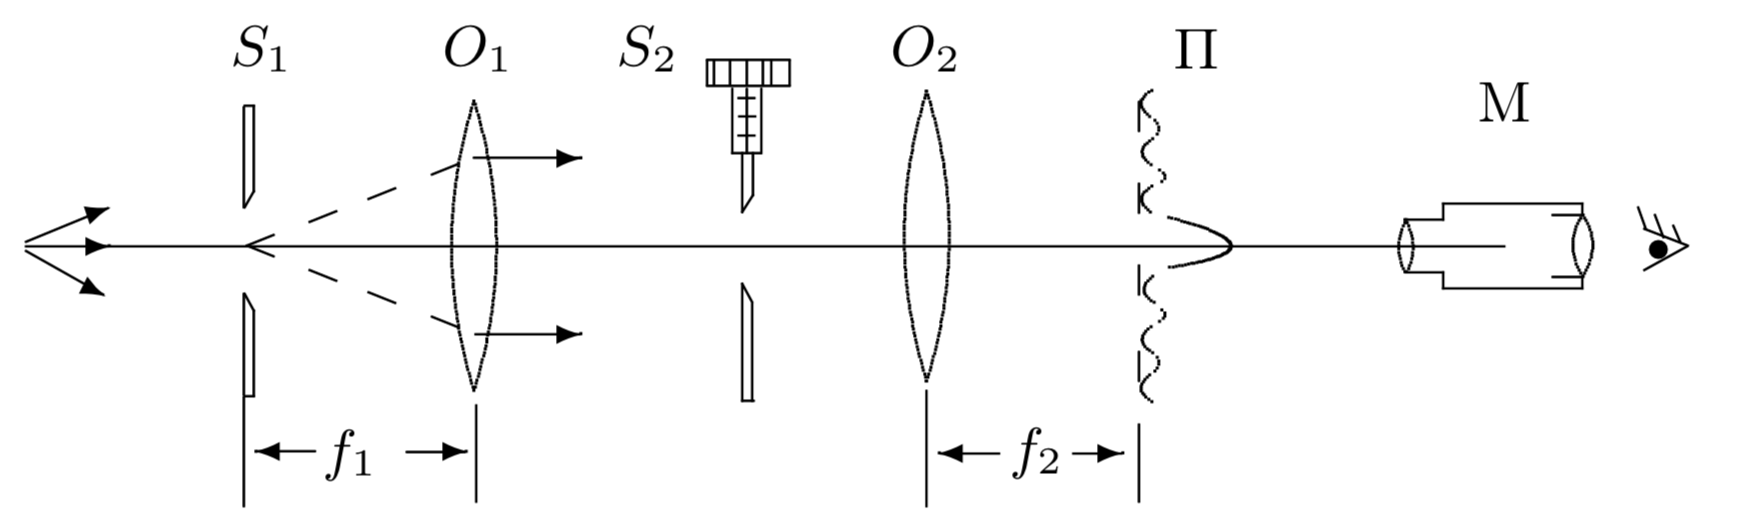
\includegraphics[width=0.8\linewidth]{b.png}
	\caption{Схема установки для наблюдени дифракции Фраунгофера}
	\label{labB}
\end{figure}

Расстояние $X_m$ тёмной полосы от оптической оси объектива $O_2$ пропорционально фокусному расстоянию $f_2$.
Получаем $X_m =\frac{f_2m\lambda}{D}$. При малых углах минимумы эквидистантны, а расстояния $\varDelta X$ между минимумами обратно пропорциональны ширине $D$ щели $S_2$.

\subsection{Дифракция Фраунгофера на двух щелях}

\begin{figure}[h!]
	\centering
	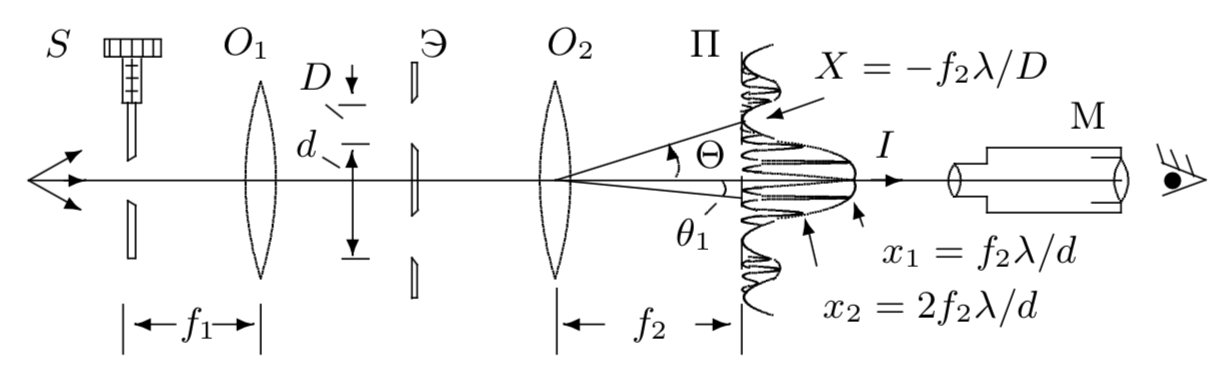
\includegraphics[width=0.8\linewidth]{c.png}
	\caption{Схема установки для наблюдния дифракции Фраунгофера на двух щелях}
	\label{labC}
\end{figure}

Если входная щель достаточно узка, то дифракционная картина в плоскости П (рис. 3) подобна той, что получалась при дифракции
на одной щели (рис. 2), однако теперь вся картина испещрена рядом дополнительных узких полос.

\section{Ход работы}
\subsection{Дифракция Френеля на щели}

\begin{enumerate}
	\item Провели натсройку приборов, собрали установку. Наблюдали дифракцию Френеля
	на щели – на ярком фоне изображения щели появляются темные полосы, количество
	которых уменьшается по мере удаления от микроскопа
	\item Сняли зависимость количества полос от расстояния до микроскопа
	
	\begin{table}[h!]
		\caption{Зависимость координаты микроскопа от числа $ n $ темных полос}
		\begin{center}
			\begin{tabular}{|c|c|c|c|c|c|}
				\hline
				m & 1 & 2 & 3 & 4 & 5 \\
				\hline
				x, мм & 23 & 14 & 11 & 9 & 8 \\
				\hline
			\end{tabular}
		\end{center}
		\label{}
		\end{table}

	\item Посчитаем зависимость ширины зон Френеля от количества и построим график зависимости по формуле (1)

	\begin{table}[h!]
		\caption{Зависимость координаты микроскопа от числа $ n $ темных полос}
		\begin{center}
			\begin{tabular}{|c|c|c|c|c|c|}
				\hline
				m & 1 & 2 & 3 & 4 & 5 \\
				\hline
				$2z_m, мм$ & 0.226 & 0.249 & 0.271 & 0.283 & 0.298 \\
				\hline
				$\delta 2z_m, мм$ & 0.002 & 0.004 & 0.006 &0.007 & 0.009 \\
				\hline
			\end{tabular}
		\end{center}
		\label{}
		\end{table}
	
		\begin{figure}[H]
			\begin{center}
			\label{graf_a}
			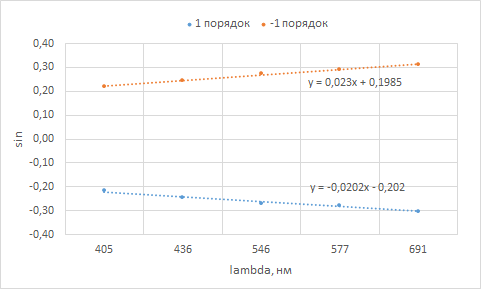
\includegraphics[scale=0.5]{гр1.png}
			\caption{График зависимости между шириной зон Френеля от количества полос}
			\end{center}
		\end{figure}

	\item Ширина щели $S_2 $ $ D = 0,310 \pm 0, 001$ мм.
	\item Теперь расчитаем ширину щели с помощью таблицы 2 и рассчитаем погрешности. \\
	$\delta x = 0.5 мм$. \\
	$\delta2z_m = 2z_m \cdot\frac{\delta x}{2x}$ \\
	$\delta D = \frac{1}{m(1 - m)}\sqrt{\sum(D_i - D)}$  $D = 0.265 \pm 0.007$ мм

	\item Построим график.
	
	\begin{figure}[H]
		\begin{center}
		\label{graf_a}
		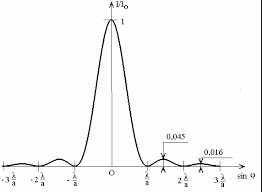
\includegraphics[scale=0.5]{d.png}
		\caption{График зависимости распределения интенсивности}
		\end{center}
	\end{figure}

	\item В начале наблюдалась дифракционная картина с одной темной плосой, далее при увеличении ширины - количество полос растет, причем возле границ - самая яркая полоса. После вместо щели установили тонкую нить, настроив микроскоп на ее резкое изображение. При удалении микроскопа от нити количество наблюдаемых нитей растет, наблюдаем четное количество темных полос.
\end{enumerate}



\section{Дифракция Фраунгофера на одной щели}
\begin{enumerate}
	\item На значительном удалении от щели, когда ширина щели становится значительно меньше ширины первой зоны Френеля, изображение щели размываетмя и возникае дифракцонная картина, называемая дифракцией ФФраунгофера.
	\item Фокусные рассояния линзы $F_2 = 13.8 $см.
	\item Добавим линзу $O_2$ и настроим микроскоп на окальную плоскость. Затем подберем ширину щели для получения дифракции. Измерим координаты нескольких минимумов, запишем в таблицу и построим график.
	\item Величина щели по винту равна $ D = 0,312 - 0,052 = 0,26 \pm 0,01 $ мм.

Измерим с помощью винта поперечного перемещения микроскопа координаты $ X_m $ нескольких дифракционных минимумов. Здесь $ x_m $ - измерения, которые затем умножаем на $ \alpha = 0,02 $ мм --- цену деления винта, т.е. $ X_m = \alpha x_m $.
Результаты занесем в табл. 2 и построим график зависимости минимумов от их номеров. 

\begin{table}[h!]
	\caption{Зависимость минимумов от их номера $ m $}
	\begin{center}
		\begin{tabular}{|c|c|c|}
			\hline
			$ x_m $ & $ X_m $, мкм & $ m $ \\
			\hline
			-2.2 & -88 & -2 \\
			-1.0 & -41 & -1 \\
			0.0 & 0 & 0 \\
			1.0 & 41 & 1 \\
			2.1 & 84 & 2 \\
			\hline
		\end{tabular}
	\end{center}
	\label{}
\end{table}

\item $tg \alpha = \frac{X_m}{m} = 42,2 \; мкм$

\begin{table}[H]
	\caption{Зависимость минимумов от их номера $ m $}
	\begin{center}
		\begin{tabular}{|c|c|c|c|c|c|}
			\hline
			m & -2 & -1 & 0 & 1 & 2 \\
			\hline
			$ D, мм $ & 0,236 & 0,253 &0,260 & 0,253 & 0,247 \\
			\hline
		\end{tabular}
	\end{center}
	\label{}
\end{table}

\item $D = \frac{f_2\cdot\lambda}{tg\alpha} = 0,25 \pm 0,01 $ мм - усредненное значение
\item $\delta D = D \frac{1}{\sqrt{m(m - 1)}}\cdot \sqrt{\sum_{i=1}^n (D_i - D)^2}$

	\begin{figure}[H]
		\begin{center}
	\label{graf_b}
	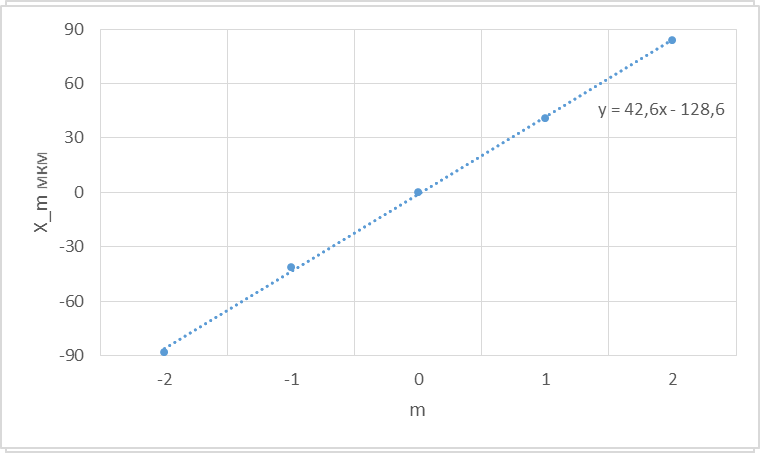
\includegraphics[scale=0.5]{гр2.png}
	\caption{График зависимость $ X_m $ минимумов от их номера $ m $}
		\end{center}
\end{figure}

\item Убедились, что смещение щели $S_2$ не приводит к сдвигу картины. При уменьшении щели масштаб картинки уменьшается, пока картинка полностью не исчезнет.
\end{enumerate}

\section{Дифракция Фраунгофера на двух щелях}

\begin{enumerate}

\item Не перемещая линз заменим $S_2$ и, слегка передвигая ее вдоль скамьи, найдем резкое изображение. Получим для 1 и 2 максимума слева и справа соответственно координаты на винте $ x_m $, а затем получим $ X_m = \alpha x_m $ аналогично предыдущему пункту. 
\item Самый левый - 2.24 мм, правый 3.68 мм, расстояние между ними 1,44 мм, расстояние между краями максимумов $\delta x = 0.08 мм$.
Отсюда $ d = f_2 \frac{\lambda}{\delta x} = 1.2$ мм. Из него получаем рассчетное число максимумов $n = \frac{2d}{D} = 12$, что совпадает с экспериментальным.

 \begin{table}[H]
	\caption{Измерения максимумов на двух щелях}
	\begin{center}
		\begin{tabular}{|c|c|c|c|c|}
			\hline 
			$m$ & -2 & -1 & 1 & 2 \\ 
			\hline 
			$x_m$ & 1,55 & 1,6 & 2,3 & 2,4 \\ 
			\hline 
			$X_m$, мм & 0,031 & 0,032 & 0,046 & 0,048 \\ 
			\hline
	\end{tabular}   
\end{center} 
\end{table}

\end{enumerate}
\section{Влияние дифракции на разрешающую способность оптического инструента.}

\begin{enumerate}
	\item Соберем схему. Поставим между линзами щель $S_2$ и, уменьшая ее ширину, наблюдаем ухудшение изображения. Подберем ширину щели так, чтобы изображения почти сливались.
	\begin{equation}
		D_0{изм} = 0.03 \pm 0.01 мм
	\end{equation}
	\item Рассчитаем $D_0$ по формуле $D_0{рас} = \frac{\lambda f_1}{b} = 0.04 \pm 0.01 $ мм. Значения сходятся в педелах погрешности.
\end{enumerate}

\section{Вывод} 
 
Мы изучили два основных типа дифракции: Френеля и Фраунгофера при разных размерах щели и провели качественные наблюдения этих явлений, а также экспериментально проверили справедливость теоретических формул.  

\end{document}